\chapter{Layer 2 Scaling: Payment Channels}
Following the idea of previous chapter, we aim to scale existing blockchain performance without changing the consensus layer. Given that the consensus protocol (layer 1) is untouched, these methods are known to afford Layer 2 scaling. Two prominent
instances are side blockchains (can handle account based systems and smart contracts) and payment channels (focused on the UTXO state management system). In this chapter, we will discuss about \textbf{payment channels}.

\section{Payment Channels}
Payment channels allow users to exchange transactions for multiple times off-chain and only broadcast the final state to the main blockchain. Users submit transactions on-chain to start the channel and handle a dispute. This reduces the load on the network and the fees for the users. \\
It locks parts of the state of the blockchain when starting a channel, processes transactions associated with this locked state in an application layer, and finally unlocks the channel with the updated state.\\\\
A UTXO system like Bitcoin consists of transactions that have inputs and outputs. Outputs serve as \textbf{locks} for a specific amount of funds, while inputs serve as keys of corresponding outputs to \textbf{unlock} the funds and transfer them between accounts.

\ex{
	\label{ex:L13_1}
	Locking and unlocking script: Pubkeyhash}{A locking script is a condition that must be satisfied to spend an output. An unlocking script is a proof that the spender meets the condition.\\
	Figure \ref{fig:L13_f1} illustrates an example of a transaction where Alice sends 1 BTC to Bob. The locking script requires that the spender provides a public key that matches the hash of Bob’s public key, and a signature that proves the ownership of the private key. The unlocking script provides these two pieces of information. The nodes then execute the scripts and check if they are valid. If they are, the transaction is confirmed and Bob can spend the output.}
\begin{figure}[h!]
	\centering
	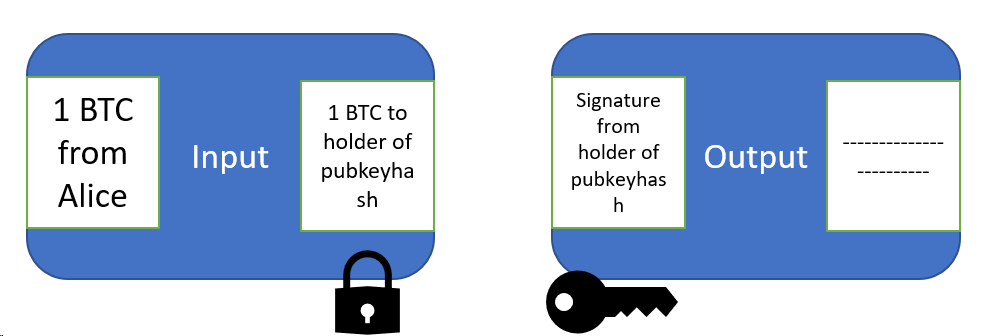
\includegraphics[width=0.7\linewidth]{Fig/13/F1}
	\caption{Example \ref{ex:L13_1} Figure}
	\label{fig:L13_f1}
\end{figure}

There are three new types of cryptographic primitives that allow "flexible locks", so that the trust can be extracted outside the blockchain :
\begin{itemize}
	\item \textbf{Multisig} : Locking transaction has to be signed by $k$ out of $n$ public keys.
	\item \textbf{Hashlock} : A hashlock is a type of cryptographic lock that can be opened by the owner of a public key (Bob) and a secret. The transaction has a locking script that contains the hash of the secret and a public key. The transaction can only be spent by Bob if he provides the secret and a signature that proves his ownership of the private key. The secret is a random value that is generated by Alice, who wants to send funds to Bob.
	\item \textbf{Timelock} : A timelock is a type of cryptographic lock that can be opened only after a certain time or block height.\\
	There are two kinds of timelocks:
	\begin{itemize}
		\item \textbf{CLTV (Check Lock Time Verify)} : transaction can only be spent after a specific block height or timestamp.
		\item \textbf{ CSV (Check Sequence Verify)} :  transaction can only be spent after a certain number of blocks have passed since the transaction was recorded in the blockchain.
	\end{itemize}
\end{itemize}

\section{One-Way Payment Channel}
One-way payment channels only allow funds to flow in one direction, from payer to recipient. For example, suppose Alice wants to pay Bob in increments of 1 BTC up to a maximum of 10 BTC. the payment channel proceeds in the following
steps:
\begin{enumerate}
	\item \textbf{Creating the channel} : \\
	Alice signs a \textbf{funding transaction} and posts it on the blockchain to
	create the channel. The funding transaction has one input with 10 BTC that Alice signs. The output can either:
	\begin{itemize}
		\item contain an address that is made from Alice and Bob’s public keys (multiaddr = GetAddrbyAccount(pk1, pk2)). It needs both Alice and Bob’s secret keys to unlock it. Neither of them can do it alone.
		\item The output has Alice’s address, and a \textbf{timelock} for the channel. If Bob is online, he can get the payment by posting a closing transaction. If not, the coins go back to Alice when the time is up.
	\end{itemize}	
	\begin{figure}[h!]
		\centering
		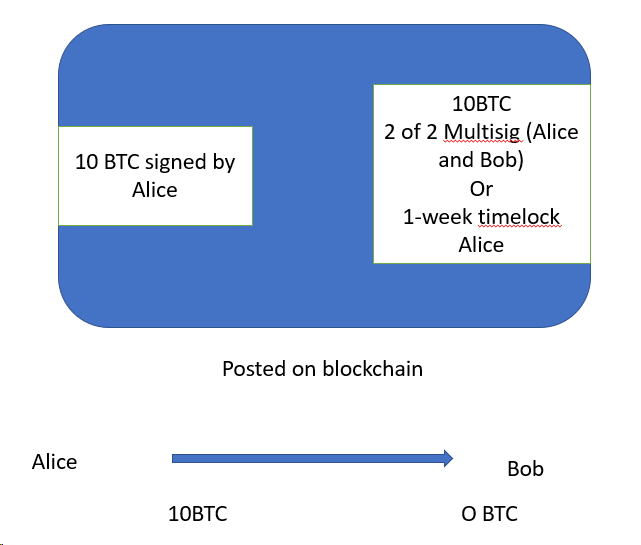
\includegraphics[width=0.3\linewidth]{Fig/13/F2}
		\caption{Funding transaction}
		\label{fig:L13_f2}
	\end{figure}
	
	\item \textbf{Updating the payments} :\\
	Each payment makes a new off-chain transaction, called a \textbf{commitment transaction}. A commitment transaction uses the same input as the funding transaction, and shows how the funds are split between Alice and Bob in the output, e.g. 9 BTC to Alice, 1 BTC to Bob.\\
	Alice can keep paying Bob like this in the channel. Every time she wants to send another 1 BTC to Bob, she makes a new commitment transaction from the same input and gives it to Bob. \\
	Bob keeps these transactions, and he can choose to post any one (but only one) of them to the blockchain to get the funds.
	\begin{figure}[h!]
		\centering
		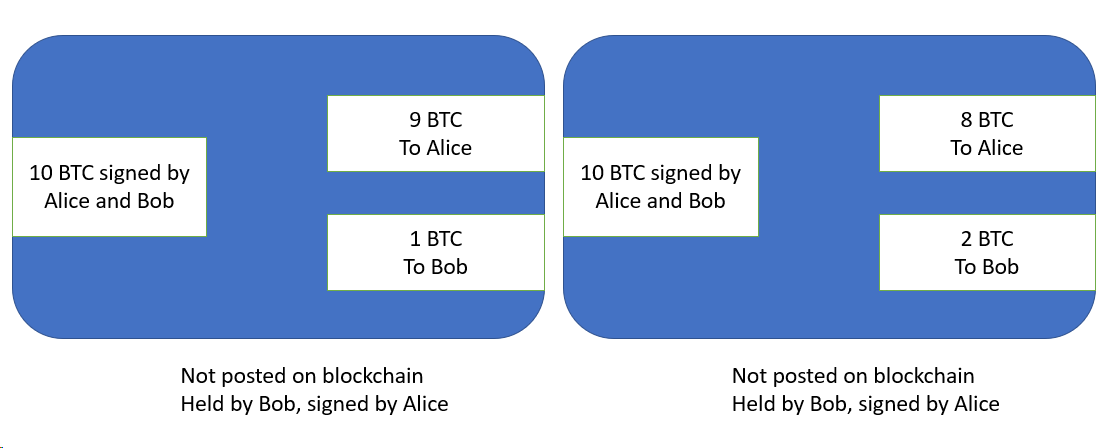
\includegraphics[width=0.6\linewidth]{Fig/13/F3}
		\caption{Commitment transaction}
		\label{fig:L13_f3}
	\end{figure}
	
	\item \textbf{Closing the channel} :\\
	To close the channel, a \textbf{closing transaction} is generated and posted on	blockchain to close the channel and update the state. There are two possible ways to close the	channel corresponding to the funding transaction:
	\begin{itemize}
		\item \textbf{Cooperative}: Bob posts a commitment transaction that he and Alice both signed with their secret keys (2-of-2 multisig). The blockchain checks the signature and matches it with the address of the funding transaction. This confirms that Alice paid Bob.
		\item \textbf{Non-cooperative}: Bob is offline and the channel runs out of time (e.g. one-day timelock). Alice posts the closing transaction on the blockchain. The transaction has Alice’s signature and a time limit that has passed. Alice gets her money back.
	\end{itemize}
\end{enumerate}

\section{Two-Way Payment Channel}
Two-way payment channels enable two parties to transfer funds to each other. Suppose now Alice
and Bob both have 5 BTC to make payments. Consider the following steps :
\begin{enumerate}
	\item \textbf{Creating the channel} : \\
	The funding transaction has two inputs, each with 0.5 BTC, one from Alice and one from Bob. The output has 1 BTC that needs both Alice and Bob’s signatures (2-of-2 multisig). Before they start paying each other, Alice and Bob make secrets and share their hashes. The opening transaction will not be signed and posted on-chain until Alice and Bob receive a
	special commitment transaction respectively. The commitment transaction here will contain
	an input with 10 BTC signed by both Alice and Bob (the output of a funding transaction), and
	two outputs. For the transaction that is held by Alice, the outputs are (1) 5 BTC to Bob,
	and (2) 5 BTC with timelock to Alice or to Bob if he knows Alice’s secret, these outputs are
	signed by Bob. Similar for Bob, the outputs are signed by Alice and contain (1) 5 BTC to
	Alice, and (2) 5 BTC with one-week timelock to Bob or to Alice if she knows Bob’s secret.
	\begin{figure}[h!]
		\centering
		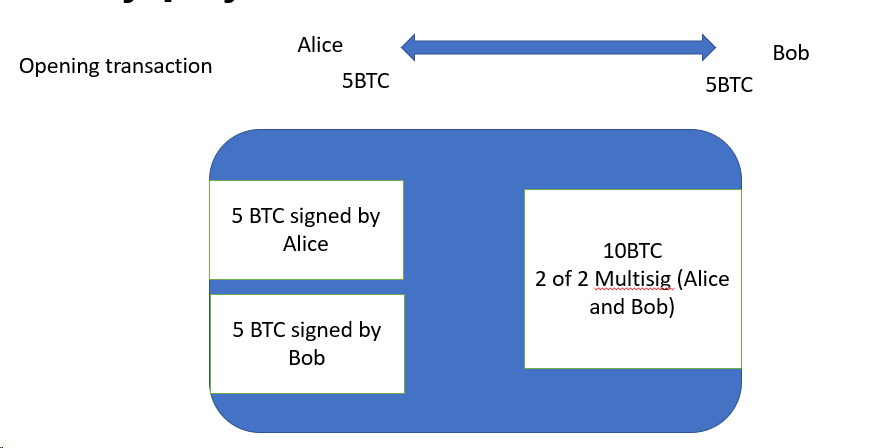
\includegraphics[width=0.4\linewidth]{Fig/13/F4}
		\caption{Two-Way payment channel}
		\label{fig:L13_f4}
	\end{figure}
	
	\item \textbf{Updating the payments} : \\
	Alice and Bob start generating a normal commitment transaction. Suppose Alice wants to send Bob 1 BTC, then she will sign a transaction with outputs: (1) 4 BTC to Alice, and 6 BTC with one-week timelock to Bob or to Alice if she knows
	Bob’s secret. For each payment, Alice and Bob will generate a new secret and exchange the older secret to ensure that the older transaction will not be posted on chain.
	\begin{figure}[h!]
		\centering
		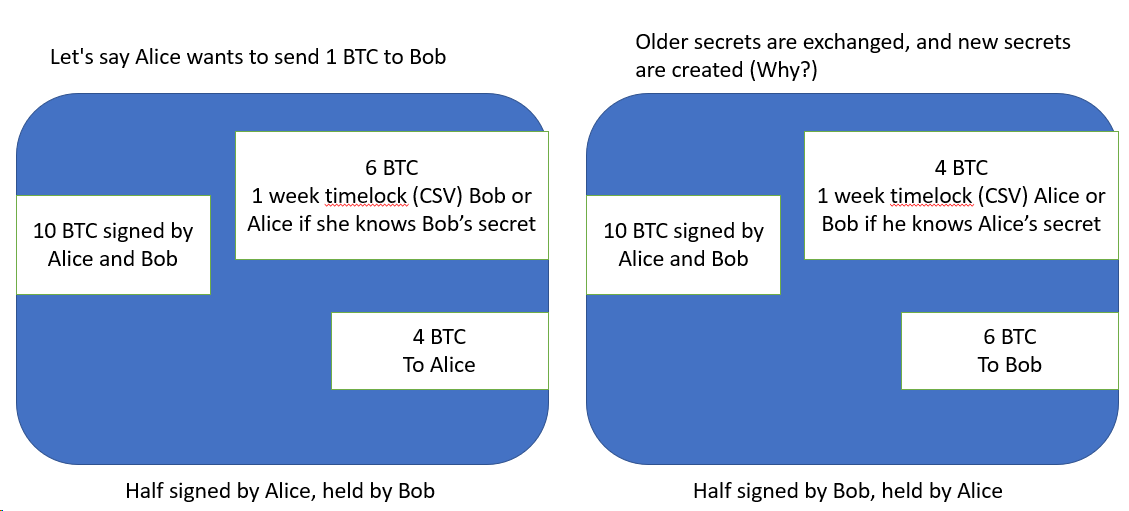
\includegraphics[width=0.5\linewidth]{Fig/13/F5}
		\caption{Commitment Transaction}
		\label{fig:L13_f5}
	\end{figure}
	
	\item \textbf{Closing the channel} : \\
	When one of the parties is offline, the channel can be closed by revealing
	any one of the commitment transactions in a non-cooperative way. And in the cooperative
	situation, Alice and Bob can create a transaction sending the settled balance to each party.
\end{enumerate}

\section{Multi-hop payment channels}
Multi-hop payment is a technique that allows users to make payments across a network of payment channels without having to establish a direct channel between them.
\subsection{Trusted multi-hop payments}
Trusted multi-hop payments allow parties who do not have a direct channel to route their payments through intermediaries who do. 
\ex{Trusted multi-hop payments}{Alice wants to pay Carol 1 BTC, but they do not have a channel between them. However, Alice and Bob have a channel, and Bob and Carol have a channel. Therefore, Alice can send 1 BTC to Bob, and Bob can forward 1 BTC to Carol, completing the payment. Alice and Carol have to trust Bob to forward the payment correctly and not steal the funds. }
\subsection{Trustless multi-hop payments using Hashlock}
The secret is a random value that is generated by the receiver of the payment and shared with the sender through a secure channel. The sender then uses the hash of the secret to lock the payment in a transaction that can only be spent by the receiver if he provides the secret. This way, the sender can ensure that the payment will not be lost or stolen.
\ex{Trustless multi-hop payments using Hashlock}{ \label{ex:L13_4.2} Alice wants to pay Carol. Carol creates a secret S and sends its hash to Alice. Alice then sends 1 BTC to Bob using hashlock, with the condition that Bob can only claim it if he knows S. Bob then sends 1 BTC to Carol using hashlock, with the same condition. Carol can then reveal S to Bob and claim her payment. Bob can then use S to claim his payment from Alice. This way, Alice can pay Carol without trusting Bob, and Bob can act as an intermediary without risking his funds. See Figure \ref{fig:L13_f6}}
\begin{figure}
	\centering
	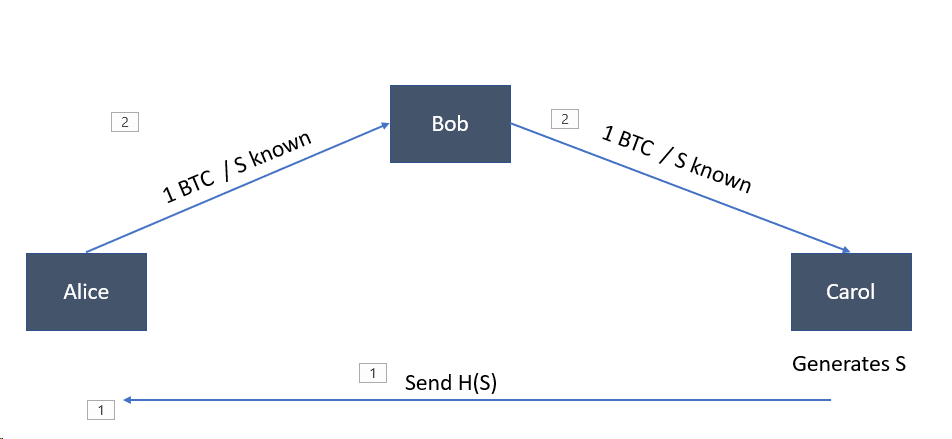
\includegraphics[width=0.6\linewidth]{Fig/13/F6}
	\caption{Trustless multi-hop payments using Hashlock}
	\label{fig:L13_f6}
\end{figure}

\subsection{Trustless multi-hop payments using Hashlock and Timelock}
Imagine the same scenario as of the Example \ref{ex:L13_4.2}. In addition to the previous transactions, now Carol also sends 1 BTC to Bob with a timelock of 1 week and also Bob sends 1 BTC to Alice with a timelock of 2 weeks. \\
Carol can claim the payment from Bob by revealing Secret, which also allows Bob to claim the payment from Alice. If Carol does not reveal Secret before a week, Bob gets his 1 BTC back. If Bob does not reveal S before 2 week, Alice gets her 1 BTC back. This way, the payment is trustless and secure.
\begin{figure}[h!]
	\centering
	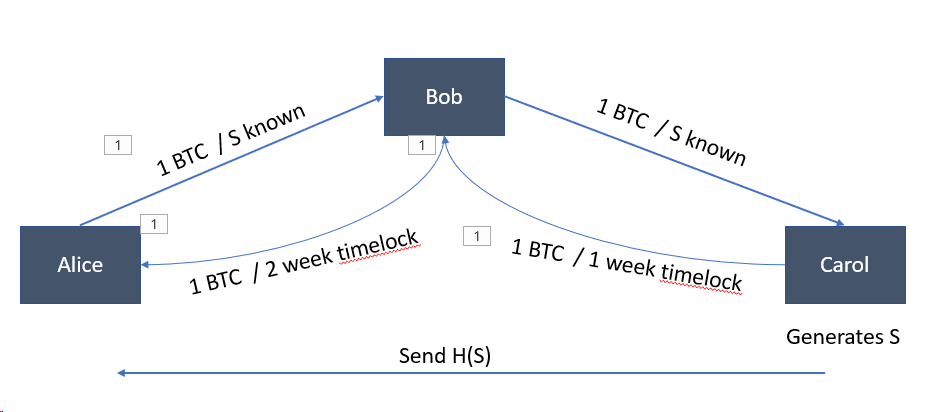
\includegraphics[width=0.6\linewidth]{Fig/13/F7}
	\caption{Trustless multi-hop payments using Hashlock and Timelock}
	\label{fig:L13_f7}
\end{figure}

\section{Payment Network}
A payment network is a system that allows users to transfer money or other assets across a network of participants. One of the challenges of designing a payment network is to enable multi hop payments, which are payments that involve more than two parties and require routing through intermediate nodes.\\\\
A lightening network is a solution for bitcoin that uses multi hop payment channels and routing to enable fast, cheap, and scalable transactions. A lightening network is a network of payment channels that are connected by nodes that can route payments between different channels.\\\\
The fee structure of the Lightning Network is based on two components:
\begin{itemize}
	\item \textbf{Base fee} : The base fee is a fixed amount of Satoshi that is charged for each payment that is forwarded through a node.
	\item \textbf{Fee rate} : The fee rate is a variable amount of Satoshi that is charged for each million Satoshi that is transferred.
\end{itemize}
The total fees are calculated as follows:
\begin{align*}
	\text{Amount}\times\text{Fee rate} + \text{Base fee}
\end{align*}
The Lightning Network fees are much lower than the on-chain fees and can enable microtransactions that are otherwise not feasible on the blockchain.\\\\
In a Lightning Network :
\begin{itemize}
	\item The total number of participating nodes is around 20,000.
	\item The total number of channels is around 85,000.
	\item The total capacity is around USD 100 million or 5,000 BTC. The capacity is the amount of bitcoin that is locked in the payment channels and can be transferred through the network.
	\item The highest capacity node is a node that has the most bitcoin locked in its channels. The highest capacity node has around 650 BTC.
\end{itemize}
The benefits of Lightning Networks are listed below:
\begin{itemize}
	\item High throughput
	\item Low latency
	\item Less fees
\end{itemize}
The list of drawbacks includes:
\begin{itemize}
	\item \textbf{Routing}: The Lightning Network relies on nodes to route payments between different channels, which can pose some challenges such as:
	\begin{itemize}
		\item \textbf{Traffic}: The network may experience congestion or delays due to high demand or low availability of nodes or channels.
		\item \textbf{Balance based}: The network may not be able to route payments that exceed the available balance or capacity of the channels involved.
		\item \textbf{Centralization} : The network may become more centralized as some nodes may have more influence or power than others due to their high capacity, connectivity, or reliability.
	\end{itemize}
	\item \textbf{Nodes need to stay online} : The nodes that participate in the network need to be online and monitor their channels to ensure the security and validity of the payments. This may create a trade-off between convenience and security for the users. Alternatively, the users may choose to outsource the monitoring of their channels to third-party services called \textbf{watchtowers}, which can prevent channel theft or fraud. However, this may also introduce trust issues or privacy risks for the users.
	\item \textbf{Capital locked in channels}: The Lightning Network requires users to lock some amount of bitcoin in their channels to enable payments. This may reduce the liquidity or availability of bitcoin for other purposes, such as saving, investing, or spending on the blockchain.
\end{itemize}